\chapter{Introducción específica} % Main chapter title

\label{Chapter2}
\label{IntroGeneral}
En este capítulo se presentan los procedimientos técnicos para la obtención de señales EEG y los métodos de extracción de características aplicados en este trabajo. Asimismo, se describen las arquitecturas de redes neuronales orientadas a la clasificación de tareas de imaginación motriz.

\section{Adquisición de datos}

El conjunto de datos seleccionado para este trabajo provino de los registros originales publicados por los autores del estudio Dreyer2023A \cite{dreyer2023large}, que presenta una base de datos de señales EEG orientada al análisis de la intención motora en sujetos sanos.

Es importante destacar que la adquisición de las señales EEG y el diseño del protocolo experimental fueron realizados por los autores del estudio original. En este trabajo no se llevó a cabo la recolección de datos, sino que se utilizó este conjunto de datos público como base para el desarrollo de los procesos de análisis, modelado y clasificación.

En el estudio original, la recolección de la actividad cerebral se realiza mediante un sistema de alta resolución que permite capturar las variaciones de potencial eléctrico en la corteza cerebral durante la ejecución de tareas mentales específicas, enfocadas en la discriminación de movimientos imaginados.

El protocolo experimental se fundamenta en un paradigma donde los participantes realizan tareas de intención de movimiento de la mano izquierda y la mano derecha sin ejecución física. Cada ensayo sigue una secuencia temporal estricta que inicia con una fase de advertencia, seguida de una señal visual que indica la dirección del movimiento imaginado. Los sujetos mantienen la actividad mental durante un intervalo de cuatro segundos, lo que permite el registro de los ritmos sensorimotores asociados a la planificación motora. Las condiciones del experimento se mantienen controladas en una habitación con aislamiento acústico para garantizar la repetibilidad de las mediciones.

\subsection{Configuración técnica y estructura del conjunto de datos}

En el estudio original, la captura de las señales la realizan mediante una distribución de 64 electrodos activos dispuestos según el sistema internacional 10-20 como puede observarse en la figura \ref{fig:electrodos}, estos se ubican sobre las áreas motoras y somatosensoriales. Esta disposición facilita la detección de los fenómenos de desincronización relacionada con eventos, los cuales resultan fundamentales para la clasificación de las tareas motrices. Los datos se registran con una frecuencia de muestreo de 500 Hz y aplican un filtro de línea de 50 Hz para reducir la interferencia eléctrica.
\begin{figure}[htpb]
	\centering
	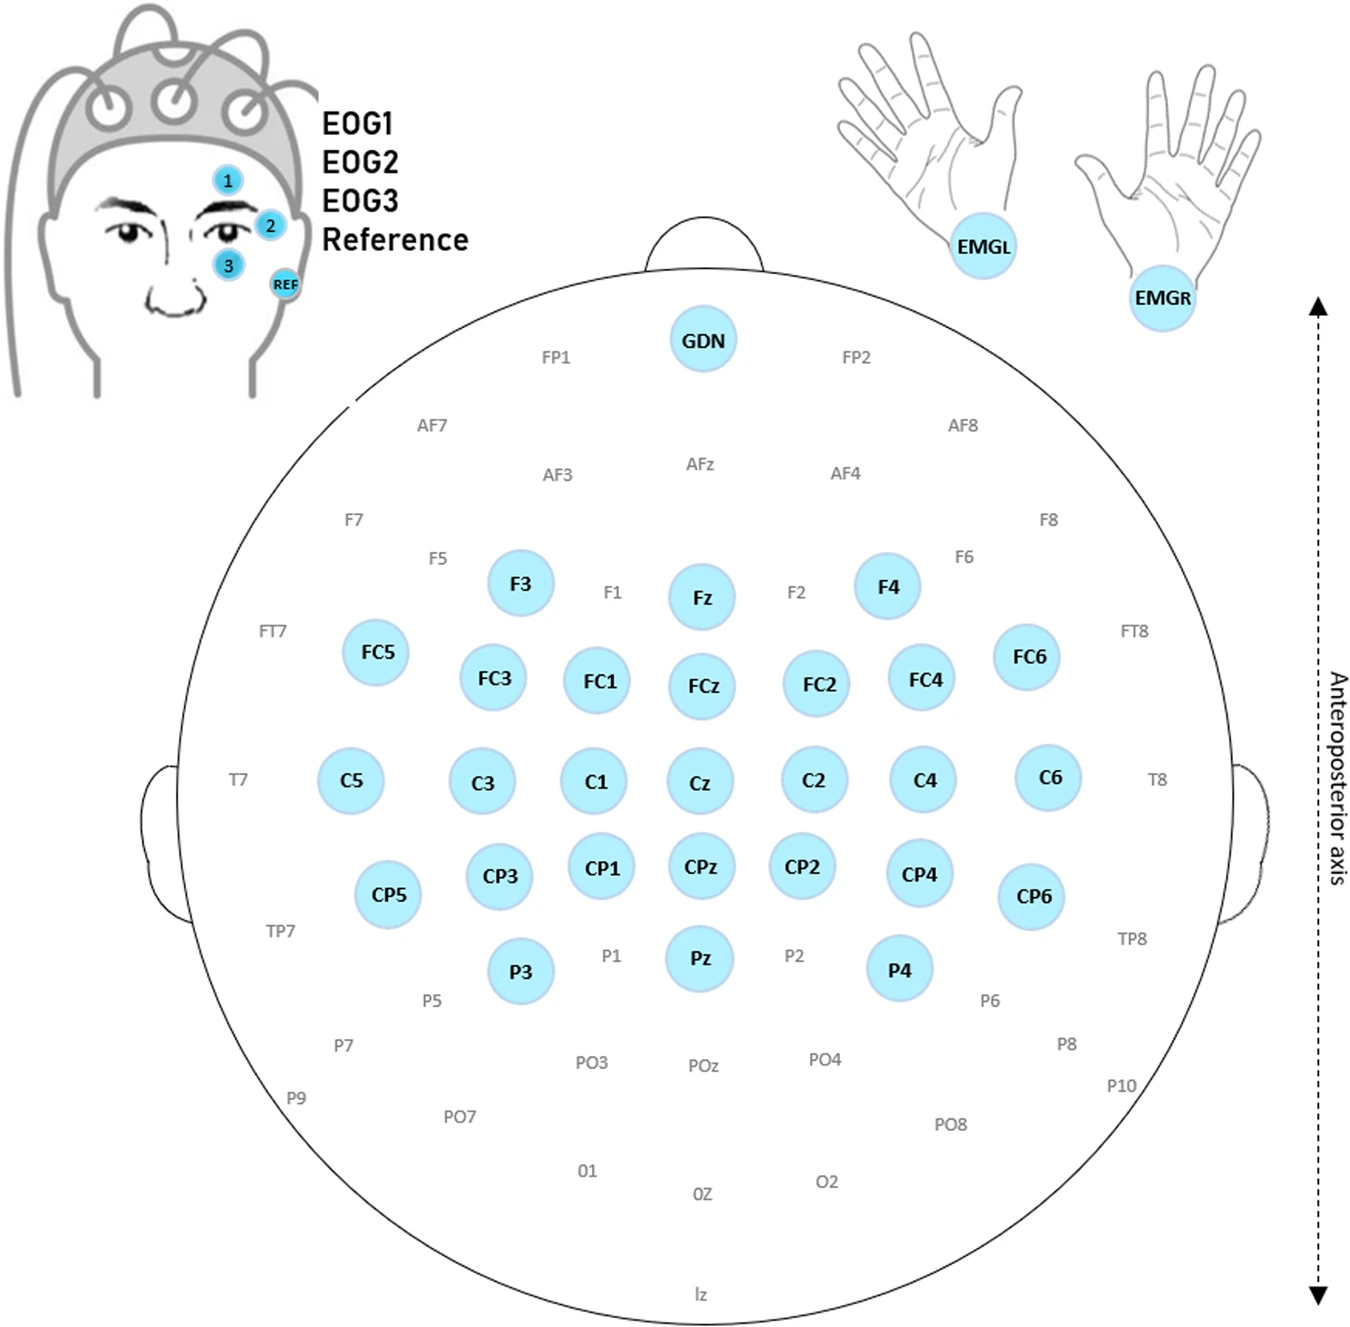
\includegraphics[scale=.2]{./Figures/EEG-10-20.jpg}
	\caption{Imagen tomada de la página oficial del procesador\protect\footnotemark.}
	\label{fig:electrodos}	
\end{figure}


% El conjunto de datos final se estructuró en registros correspondientes a 60 participantes sanos. Gracias a la integración con la biblioteca MOABB, se logró una segmentación uniforme de los ensayos, permitiendo que cada archivo incluyera las etiquetas de clase para la mano izquierda y la mano derecha de manera consistente. Esta organización facilitó el tratamiento digital de la información en la infraestructura en la nube, asegurando la integridad de las señales antes del proceso de entrenamiento de los modelos.

En la tabla \ref{tab:dataset-dreyer} se presentan las especificaciones técnicas que caracterizan al conjunto de datos utilizado en este trabajo, se destaca la cantidad de participantes, la duración de cada ensayo, el número de ensayos por clase y la calidad de las señales obtenidas. Esta información es crucial para comprender el contexto en el que se desarrolló el modelo de clasificación de imaginación motriz y para evaluar su desempeño en función de las características del conjunto de datos.

\begin{table}[h]
	\centering
	\caption[dataset dreyer]{Especificaciones técnicas del conjunto de datos Dreyer2023A.}
	\begin{tabular}{L{8cm} L{4cm}}
		\toprule
		\textbf{Parámetro} & \textbf{Valor} \\
		\midrule
		Número de sujetos           	& 60 \\
		Número de canales EEG        & 27 \\
		Número de clases de imaginación motriz 	& 2 (mano izquierda, mano derecha) \\
		Frecuencia de muestreo  		& 500 Hz \\
		Duración de ensayo  		    & 5 s \\
		Runs por sujeto				& 6 \\
		Ensayos por clase por sujeto & 20 \\
		\bottomrule
	\end{tabular}
	\label{tab:dataset-dreyer}
\end{table}

\section{Métodos tradicionales para EEG y extracción automática de características}
Tradicionalmente, la decodificación de la imaginación motriz se fundamenta en el uso de algoritmos de aprendizaje automático o Machine Learning combinados con una etapa crítica de ingeniería de rasgos manual.

El método tradicional generalizado consiste en la aplicación de CSP. Esta técnica se basa en la descomposición de las señales para maximizar la varianza entre clases, que facilita la separación de los estados mentales de movimiento \cite{riascos2024machine}. Tras la extracción de estos patrones, se emplean clasificadores de baja complejidad como el análisis discriminante lineal o LDA (del inglés, \textit{Linear Discriminant Analysis}) y las máquinas de vectores de soporte o SVM (del inglés, \textit{Support Vector Machines}). Si bien estos métodos demuestran eficacia en entornos controlados, presentan una alta sensibilidad a la colocación de los electrodos y requieren un ajuste experto de las bandas de frecuencia para cada sujeto.

Frente a estas limitaciones, el avance hacia el aprendizaje profundo o \textit{Deep Learning} ha permitido el desarrollo de modelos capaces de realizar la extracción automática de características. A diferencia de los esquemas clásicos, estas arquitecturas aprenden representaciones jerárquicas directamente a partir de los datos crudos, se reduce la necesidad de una ingeniería de rasgos manual.

Sin embargo, diversos estudios han señalado que la calidad de la adquisición de las señales EEG continúa siendo un factor determinante en el desempeño de estos modelos. Una configuración deficiente en la toma de muestras o una inadecuada colocación de los sensores puede introducir artefactos que las redes neuronales interpretan erróneamente como patrones fisiológicos, que afecta la robustez de la predicción. Por lo tanto, aunque los modelos de aprendizaje profundo contengan la capacidad de identificar características complejas, su desempeño depende en gran medida de la calidad y fidelidad de las señales de entrada.


En la tabla \ref{tab:comparacionmetodos} se presenta una comparación entre los métodos tradicionales de procesamiento de EEG y las técnicas de aprendizaje profundo. Estas destacan sus características, ventajas y limitaciones en el contexto del análisis de señales EEG para la clasificación de tareas de imaginación motriz.

\begin{table}[H]
	\centering
	\caption[Comparación entre modelos]{Comparación entre métodos tradicionales y modelos de aprendizaje profundo para el análisis de EEG.}
	\begin{tabular}{L{3cm} L{4cm} L{4cm}}
		\toprule
		\textbf{Característica} & \textbf{Métodos Tradicionales (CSP, SVM, LDA)} & \textbf{Aprendizaje Profundo (CNN, EEGNet)} \\
		\midrule
		Extracción de rasgos & Manual y basada en conocimiento experto. & Automática a partir de los datos de entrada. \\
		Sensibilidad al ruido & Muy alta, requiere filtros manuales estrictos. & Moderada, depende de la calidad del dato. \\
		Manejo de datos & Requiere segmentación y filtrado previo. & Procesamiento con preprocesamiento mínimo. \\
		Rendimiento & Limitado ante señales no estacionarias. & Mayor robustez y escalabilidad. \\
		Dependencia & Alta dependencia de calibración por sujeto. & Posibilidad de aprendizaje transferido. \\
		\bottomrule
	\end{tabular}
	\label{tab:comparacionmetodos}
\end{table}

\section{Arquitecturas de redes neuronales para EEG en imaginación motriz}

Las CNN se consolidan como una de las herramientas más eficaces para la extracción de características. Mediante el uso de filtros de convolución, estas redes permiten identificar patrones de activación en regiones específicas de la corteza motora, que simula de manera automática el comportamiento de los filtros espaciales tradicionales. Por ello, El uso de las CNN facilita la detección de cambios en la amplitud de los ritmos sensorimotores asociados a la intención de movimiento de las extremidades. 

Por otro lado, para el análisis de la dinámica temporal de las señales EEG, las redes neuronales recurrentes o RNN (del inglés, \textit{Recurrent Neural Networks}), específicamente las unidades de memoria de largo corto plazo o LSTM (del inglés, \textit{Long Short-Term Memory}) y las unidades recurrentes calificadas o GRU (del inglés, \textit{Gated Recurrent Units}) permiten modelar la evolución de la señal a lo largo del tiempo, estas utilizan mecanismos de puertas para retener información relevante y descartar el ruido transitorio. Mientras que las LSTM emplean una estructura compleja para gestionar la memoria a largo plazo, las GRU ofrecen una alternativa más eficiente en términos computacionales, que mantienen un rendimiento competitivo en la clasificación de series temporales de EEG.


Por último, los enfoques híbridos han sido ampliamente utilizados para integrar las ventajas de distintos modelos en el análisis de señales EEG. En particular, las arquitecturas de tipo CNN-LSTM combinan la capacidad de las redes convolucionales para extraer características espaciales con la habilidad de las redes recurrentes para modelar dependencias temporales \cite{zhang2021eeg}.

En este tipo de arquitecturas, las capas convolucionales permiten identificar patrones relevantes en la distribución espacial de los electrodos, mientras que las capas recurrentes procesan la evolución temporal de dichas características. Esta combinación resulta adecuada para el manejo de la alta dimensionalidad de las señales EEG, que facilita la construcción de representaciones robustas previas a la etapa de clasificación.


El enfoque híbrido y las arquitecturas de redes neuronales aplicadas al análisis de señales EEG, se puede observar en la figura \ref{fig:arquitecturas}, donde se ilustra la estructura general de cada modelo y su aplicación específica en el contexto de la clasificación de tareas de imaginación motriz, se destacan las capas de procesamiento y la forma en que cada arquitectura aborda la extracción de características espaciales y temporales para mejorar la precisión de la predicción de la intención motora a partir de señales EEG.

\begin{figure}[htpb]
	\centering
	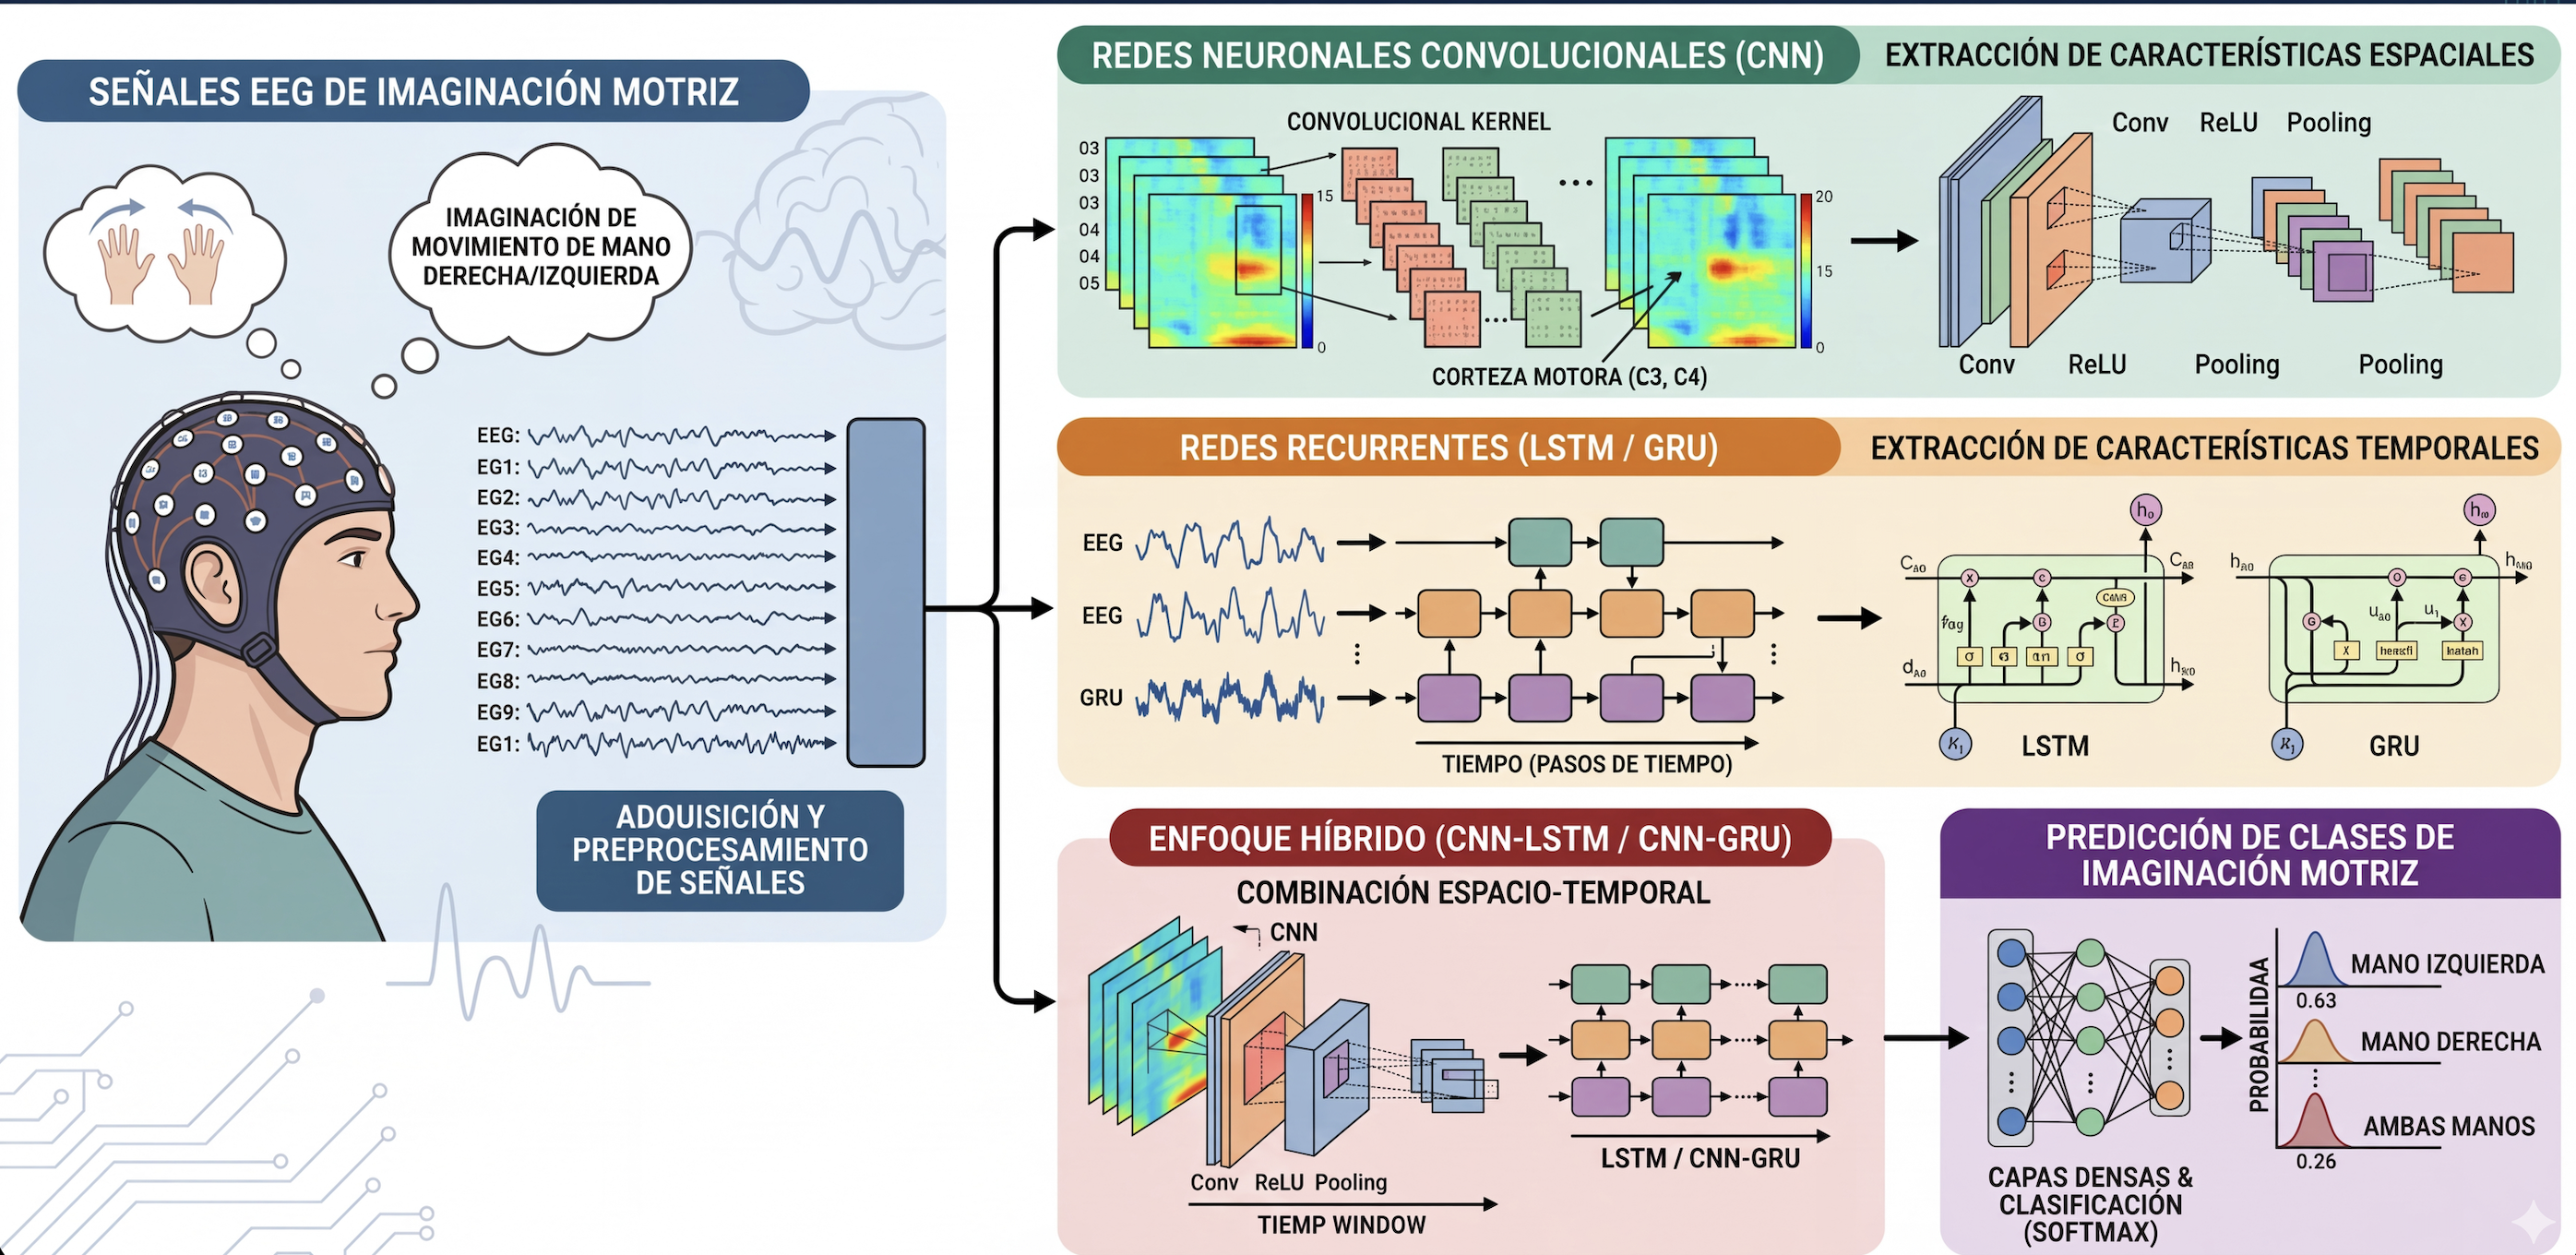
\includegraphics[scale=.26]{./Figures/redes-neuronales-eeg.png}
	\caption{Estructura general de los modelos y su aplicación en la clasificación
de tareas de imaginación motriz.}
	\label{fig:arquitecturas}	
\end{figure}


En la tabla \ref{tab:comparacionarquitecturas} se presenta una comparación técnica entre las arquitecturas de redes neuronales aplicadas al análisis de señales EEG, se destaca las características, ventajas y limitaciones en el contexto de la clasificación de tareas de imaginación motriz. Esta comparación proporciona una visión integral de cómo cada enfoque contribuye al procesamiento de las señales EEG y a la mejora del rendimiento en la decodificación de la intención motora.
\begin{table}[h]
	\centering
	\caption[Comparación entre arquitecturas]{Comparación entre arquitecturas CNN, LSTM y CNN-LSTM aplicadas al análisis de señales EEG.}
	\begin{tabular}{L{2.5cm} L{3.5cm} L{3.5cm} L{3.5cm}}
		\toprule
		\textbf{Característica} & \textbf{CNN} & \textbf{LSTM / GRU} & \textbf{CNN-LSTM} \\
		\midrule
		Tipo de procesamiento 
		& Espacial (filtros convolucionales)
		& Temporal (modelado secuencial) 
		& Espacial + temporal combinado \\

		Extracción de características 
		& Automática en dominios espaciales locales 
		& Basada en dependencias temporales 
		& Extracción jerárquica espacio-temporal \\\\

		Manejo de dependencias temporales 
		& Limitado 
		& Alto (memoria de corto y largo plazo) 
		& Alto (integrado con características espaciales) \\\\

		Complejidad computacional 
		& Moderada 
		& Alta 
		& Alta \\

		Robustez frente a ruido 
		& Moderada 
		& Moderada 
		& Alta (por integración de representaciones) \\\\

		Ventaja principal 
		& Detección de patrones espaciales en electrodos 
		& Modelado de dinámica temporal de la señal 
		& Captura conjunta de patrones espaciales y temporales \\\\

		Limitación principal 
		& No modela secuencias largas 
		& Alto costo y entrenamiento más complejo 
		& Mayor complejidad y necesidad de ajuste fino \\

		Aplicación en EEG 
		& Identificación de activación cortical localizada 
		& Análisis de evolución temporal de ritmos cerebrales 
		& Clasificación integral de tareas de imaginación motriz \\

		\bottomrule
	\end{tabular}
	\label{tab:comparacionarquitecturas}
\end{table}
\footnotetext{Imagen generada por inteligencia artificial.}
